\documentclass{article}

% Formato de página
\usepackage[letterpaper, margin = 1.5cm]{geometry}

% Más opciones para enumerar
\usepackage{enumitem}

% Manejo de imágenes
\usepackage{graphicx}
\usepackage{wrapfig}
\graphicspath{{img/}}

\begin{document}
    \title{
        Fundamentos de bases de datos \\
        Tarea 3 \\
        Modelo Relacional
    }
    \author{
        Díaz Gómez Silvia \\
        Eugenio Aceves Narciso Isaac \\
        Quiroz Castañeda Edgar
    }
    \date {
        22 de marzo del 2019    
    }
    \maketitle

    \section{Preguntas de repaso}
    \begin{enumerate}[label = \alph*.]
        \item ¿Qué es una \textbf{relación} y qué características tiene?
        \item ¿Qué es un \textbf{esquema de relación}?
        \item ¿Qué es una \textbf{llave primaria} ¿qué es una \textbf{llave 
        candidata}? ¿qué es una \textbf{llave mínima}? ¿qué es una \textbf{super
        llave}
        \item ¿Qué restricciones impone una \textbf{llave primaria} y una llave 
        foránea al modelo de dato relacional?
        \item Investiga cómo se traducen las \textbf{categorías} (presentes en
        el \textbf{modelos E/R}) al \textbf{modelos relacional}. Proporciona un 
        ejemplo.
    \end{enumerate}

    \section{Modelo relacional}
    Traduce el siguiente modelo \textbf{Entidad/Relación} a su correspondiente 
    \textbf{Modelo Relacional}:
    
    \begin{center}
        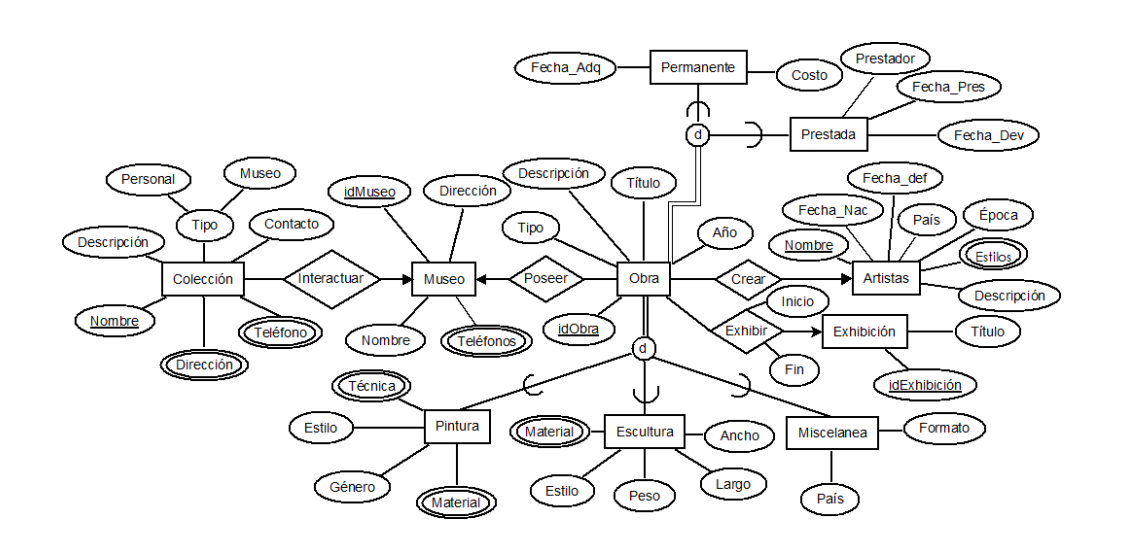
\includegraphics[width=1\textwidth]{er1.png}
    \end{center}
        
    \section{Modelo relacional}
    Traduce s su correspondiente \textbf{Modelo Relacional} el problema del 
    \textbf{Sistema de Información Geográfica (Tarea 1)}. Se realizaste alguna
    modificación a tu diseño orignal (para mejorarlo) indica los cambios hechos 
    y la justificación de los mismos.\\
    En cualquier caso, deberás mostrar el \textbf{diagrama E/R} y su
    correspondiente traducción. Es importante que muetres tanto las 
    \textbf{restricciones de entidad} como las de \textbf{integridad referencial}.


    \section{Lectura}
    Leer el artícula \textbf{Codd's 12 Rules for a RDBMS}. Explica con tus 
    propias palabras cada una de las 12 reglas de \textbf{Codd}.\\
    Indica por qué consideras que son importantes y si, hasta el momento de lo 
    comentado en el curso, sería posible que un \textbf{SMBD} pudiera cumplir 
    enteramente con lo que ahí se propone.
\end{document}